\subsection{Inference on M2}
To test our performance, we apply our method to the SDSS image of M2 found in run 2583, camcol 2, and field 136. This globular cluster was also imaged during the ACS Globular Cluster Survey CITE using the Hubble Space telescope (HST), which has $\approx20$ times the angular resolution of the Sload telescope. Thus, we use the catalog reported by the Hubble survey as ground truth to validate our catalog. 

We focus on a specific $100 \times 100$ subimage of M2 that \cite{Portillo_2017, Feder_2019} cataloged using MCMC. This subpatch is located $\approx2$ arcseconds away from the heavily saturated core of the cluster; even in this subpatch, the HST catalog reports $\approx 1000$ stars brighter than the 22nd magnitude in its F606W band. 

The metrics we examine are the true positive rate (TPR) and the positive predicted value (PPV). 
In the context of cataloging, TPR is defined as the proportion of stars in the HST catalog that had a match in our catalog; PPV is the proportion of stars in our catalog that had a match in the HST catalog. 
Like \cite{Portillo_2017, Feder_2019} a match is defined when the estimated location and the HST location is within 0.75 pixels (TODO: results actually right now are for 0.5 pixels), and the estimated r-band flux and the HST flux is within half a magnitude. 

We compare our method with the MCMC procedure of \cite{Feder_2019} and DAOPHOT catalog of M2 reported in~\cite{An_2008_m2}. 
For our method and \cite{Feder_2019}, we use the $r$ and $i$ bands (TODO: how does DAOPHOT handle bands).
We initialize our background an and the PSF parameters at the SDSS estimates. We compare running only the sleep phase, using the SDSS estimates, versus running two cycles of wake-sleep. 

In table~\ref{tab:summary_stats}, we display summary statistics, including the TPR and PPV. To compute summary statistics on our method, we use the catalog produced by our MAP estimates. For \cite{Feder_2019}, each MCMC sample results in a catalog, the collection of which they call the {\itshape ensemble catalog}. To compute summary statistics for \cite{Feder_2019}, we computed summary statistics for each catalog in the ensemble, and averaged over the ensemble catalog. We find that DAOPHOT grossly underestimates the number of stars in this submimage. Our wake-sleep procedure predicts nearly three times as many stars, while only suffering a decrease in PPV of 4\%. Conversely, \cite{Feder_2019} predicts roughtly 50\% more stars than our method, without significant gains in the TPR. We combine TPR and PPV into one statistic using the F1 score, defined as the geometric average between TPR and PPV and find that our wake-sleep method outperforms both \cite{Feder_2019} and DAOPHOT. 

% \begin{table}[!tb]
% \centering
% \caption{Performance metrics on M2.
% For probabilistic methods (StarNet and PCAT)
% the ``\#stars" column refers to the mean number of stars under the (approximate) posterior, while the right-most column displays the 5-th and 95-th percentiles under the posterior. }
% \label{tab:summary_stats}
% \begin{tabular}{l|ccc|cc}
% \toprule
%      Method &   TPR &   PPV &  F1 score &  \#stars & (q-5\%, q-95\%)\\
% \midrule
%     DAOPHOT &  0.20 &  0.63 &      0.30 &     295 & -- \\
%        PCAT &  0.56 &  0.40 &      0.47 &    1672 & (1664, 1680)\\
%  Sleep-only &  0.51 &  0.47 &      0.49 &    1292 & (1260, 1324)\\
%  Wake-sleep &  0.51 &  0.60 &      0.55 &     1014 & (987, 1041)\\
%      %Hubble &  1.00 &  1.00 &      1.00 &     1114 & -- %\\
% \bottomrule
% \end{tabular}
% \end{table}

\begin{table}[!tb]
\centering
\caption{Performance metrics on M2.
For probabilistic methods (StarNet and PCAT)
the ``\#stars" columns provide the mean along with the 5th and 95th percentiles
for the number of stars under the (approximate) posterior,
The number of stars in the Hubble catalog is 1114. }
\label{tab:summary_stats}
\begin{tabular}{l|ccc|cc}
\toprule
& & & & \multicolumn{2}{c}{\#Stars} \\
     Method &   TPR &   PPV &  F1 score &  mean & (q-5\%, q-95\%)\\
\midrule
    DAOPHOT &  0.20 &  0.65 &      0.31 &     357 & -- \\
       PCAT &  0.55 &  0.37 &      0.44 &    1672 & (1664, 1680)\\
 StarNet (our) &  0.53 &  0.48 &      \textbf{0.50} &    1462 & (1430, 1497)\\
\bottomrule
\end{tabular}
\end{table}


In figure~\ref{fig:summary_stats}, we display the TPR and PPV as a function of magnitude. 
Our method and \cite{Feder_2019} exhibit similar TPR across all magnitudes, and are 
uniformly better than DAOPHOT. Wake-sleep exhibits a PPV that is higher than \cite{Feder_2019} for all magnitudes, though DAOPHOT shows better PPV at the smaller magnitudes. 

\begin{figure}[h]
    \centering
    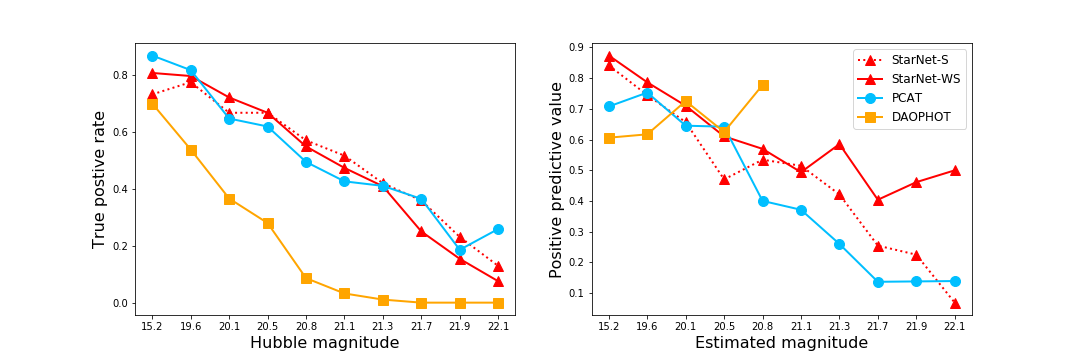
\includegraphics[width=0.99\textwidth]{figures/summary_statistics_m2.png}
    \caption{True positive rate and positive predicted value of various cataloging
    procedures on M2, plotted against magnitude percentile.
    Smaller magnitudes correspond to brighter stars. }
    \label{fig:summary_stats}
\end{figure}

In figure~\ref{fig:example_subimages}, we display four $10\times10$ subimages, and plot 
our MAP catalog against the Hubble catalog. We also display the catalog from one sample of \cite{Feder_2019} and the DAOPHOT catalog. 

\begin{figure}[h]
    \centering
    \vspace{-3cm}
    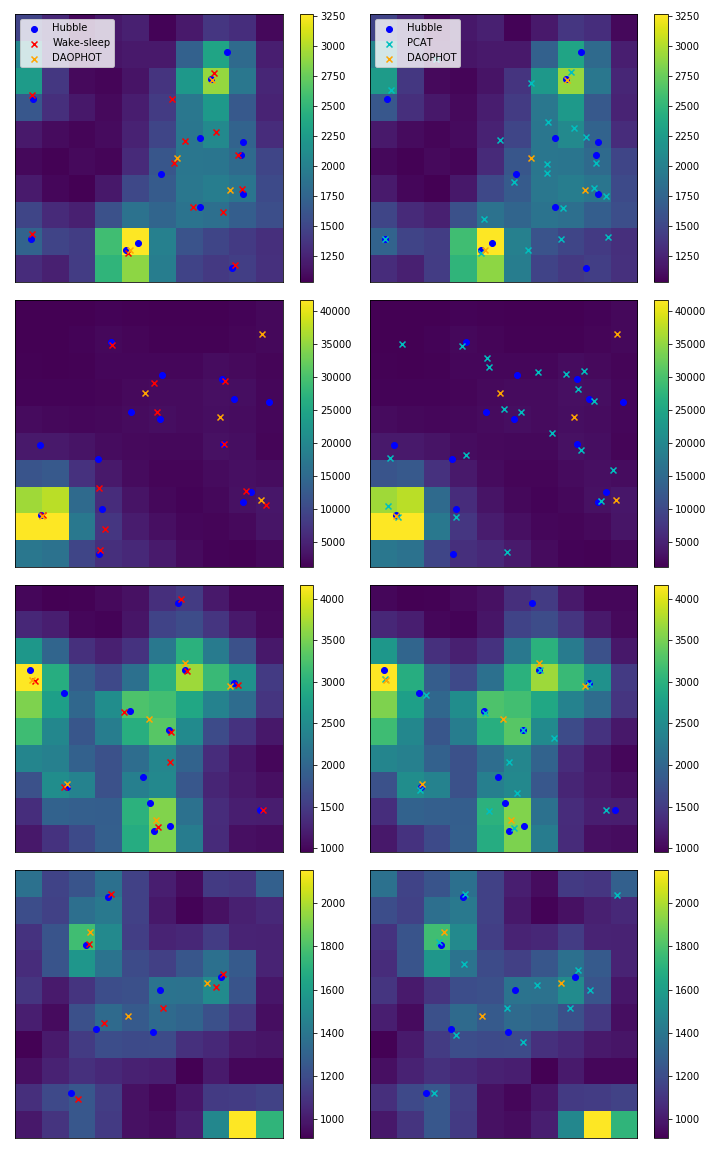
\includegraphics[width=0.8\textwidth]{figures/example_subimages.png}    
    \vspace{-3cm}
    \caption{Estimated catalogs on four 10$\times$10 subimages from 
    M2. Blue dots are Hubble stars brighter than the 22nd magnitude. 
    Starnet, Portillos, and DAOPHOT estimated stars are in 
    red, cyan, and orange x's, respectively. }
    \label{fig:example_subimages}
\end{figure}


In figure~\ref{fig:example_subimages_sampled}, we display the sampled catalogs from both our wake-sleep approximate posterior as well as from \cite{Feder_2019}. Assuming the MCMC 
of \cite{Feder_2019} converged to the true posterior, we see that our uncertainty estimates 
are generally larger. This is expected from section~\ref{sec:kl_q_p}

\begin{figure}[h]
    \centering
    \vspace{-3cm}
    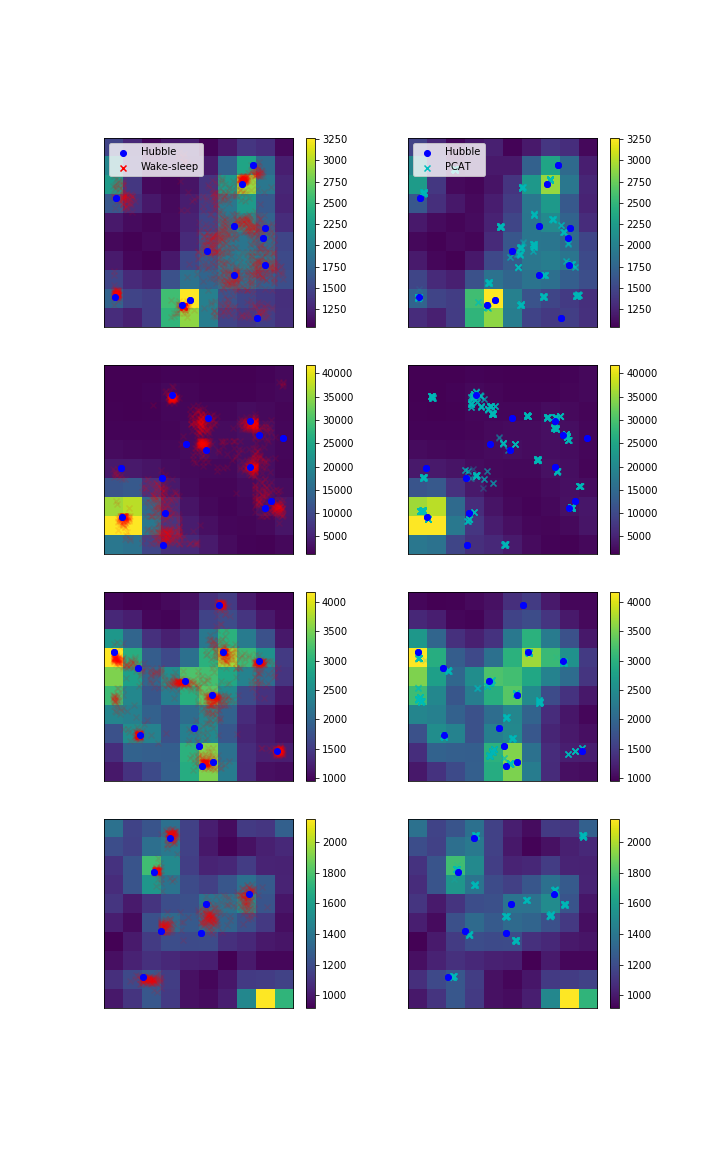
\includegraphics[width=0.8\textwidth]{figures/example_subimages_samples.png}    
    \vspace{-3cm}
    \caption{Four 10$\times$10 subimages from 
    M2. Blue dots are Hubble stars brighter than the 22nd magnitude. 
    We print display the posterior samples from our variational 
    posterior (left) and from the MCMC chain of Portillos (right). }
    \label{fig:example_subimages_sampled}
\end{figure}

\begin{figure}[h]
    \centering
    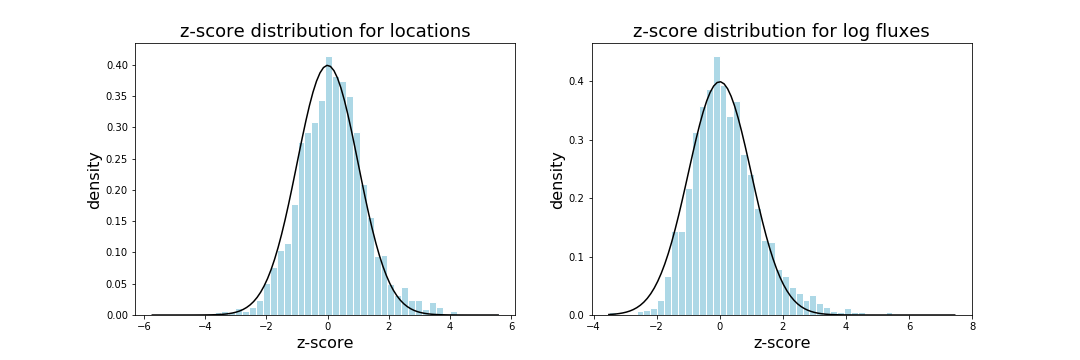
\includegraphics[width=0.99\textwidth]{figures/z-score_calibration.png}    
    \caption{The calibration of uncertainties in our variational posterior. Conditional on the true number of stars, we compute the z-score of the true location or log flux evaluated at our 
    variational posterior. }
    \label{fig:z-score_calibration}
\end{figure}


\begin{figure}[h]
    \centering
    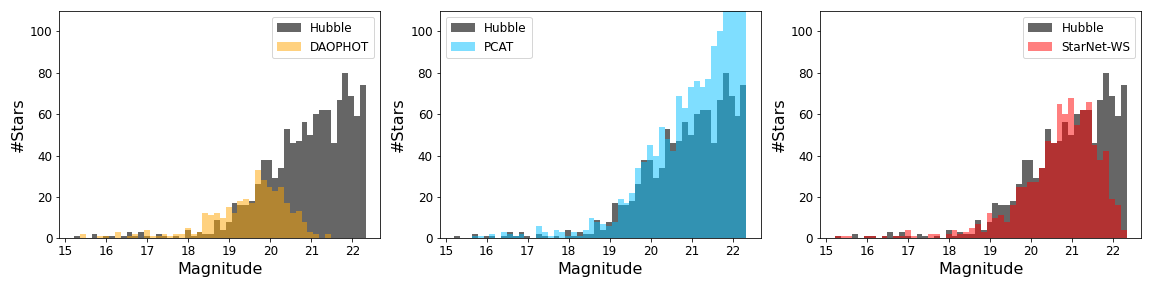
\includegraphics[width=0.99\textwidth]{figures/luminosity_fun.png}
    \caption{Source magnitude histograms on M2. }
    \label{fig:luminosity_fun_m2}
\end{figure}

\begin{figure}[h]
    \centering
    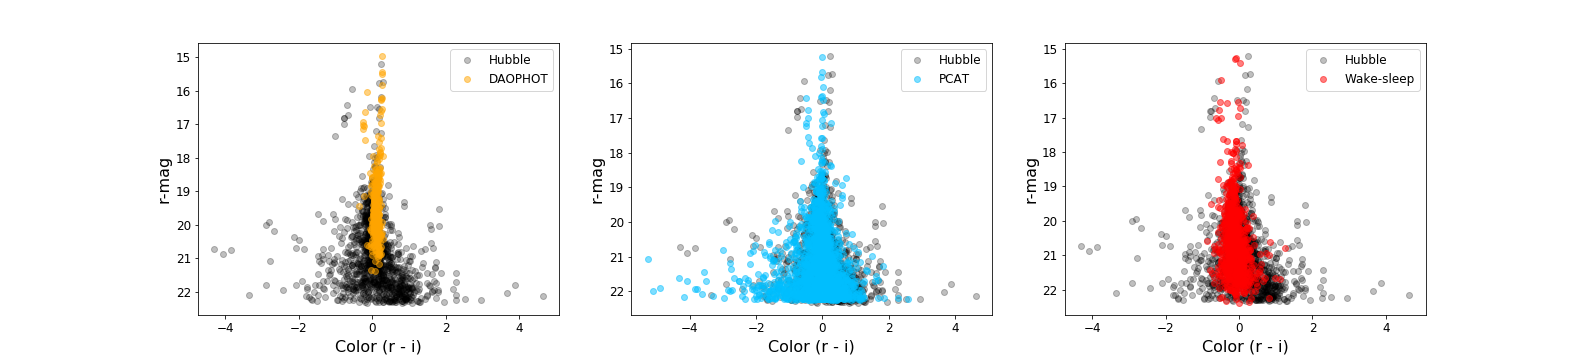
\includegraphics[width=0.99\textwidth]{figures/cmd.png}
    \caption{Color magnitude diagrams on M2. }
    \label{fig:cmd_m2}
\end{figure}


\subsection{Estimation of model parameters}
\input{tables/chi_sq_stats.txt}

\begin{figure}[h]
    \centering
    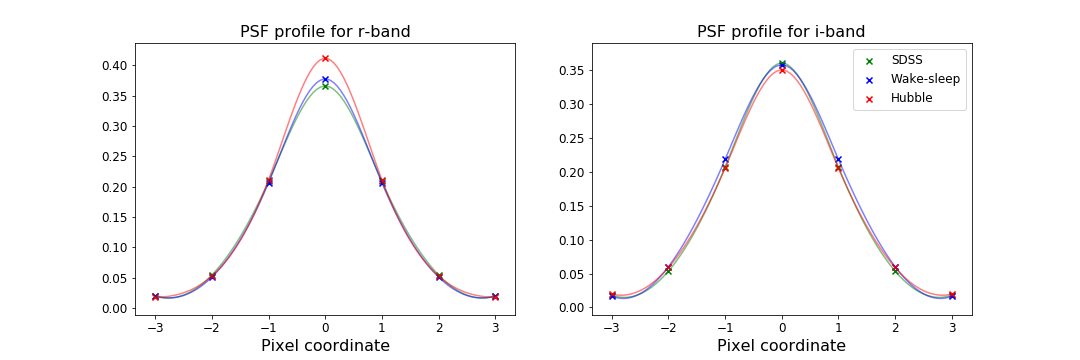
\includegraphics[width=0.99\textwidth]{figures/psf_profiles.png}
    \caption{Estimated versus true PSF profiles on M2. The Hubble PSF was
    obtained by optimizing the likelihood conditioned on locations and fluxes
    from the Hubble catalog. }
    \label{fig:psf_profiles}
\end{figure}


% \multicolumn{1}{p{5cm}}{\raggedleft Chi sq. \\ (with Hubble back.)}
% \caption{
% Chi-squared statistics for SDSS, wake-sleep, and Hubble estimated model parameters.
% The chi-squared statistic is defined as
% $\sum_{bij}\frac{([\text{obs.image}]_{bij} - [\text{recon.image}]_{bij})^2}{[\text{recon.image}]_{bij}}$.
% In the middle column, ``model parameters" refer to both background and PSF.
% In the right column, we fix the background to the Hubble estimate, and examine
% chi-squared statistics as the PSF varies.}
